\chapter{Teknologi}
I dette afsnit undersøges Ultralyds Robotarmen ud fra et teknologisk perspektiv. Den teknologiske løsning Ultralyds Robotarm består af:
\begin{itemize}
\item UR3 Robotarm fra Universal Robots incl. software til styring af denne
\item Stativ til robotten
\item Joystick
\item Computer
\item Holder til ultralydsprobe
\end{itemize}
Denne løsning skal kobles til det allerede eksisterende udstyr. Derfor er produktet en add-on løsning, hvilket betyder at produktet skal købes udover det almindelige ultralydsscanningsudstyr. Se bilag --- (ØKONOMI)
\begin{figure}[H]\centering
	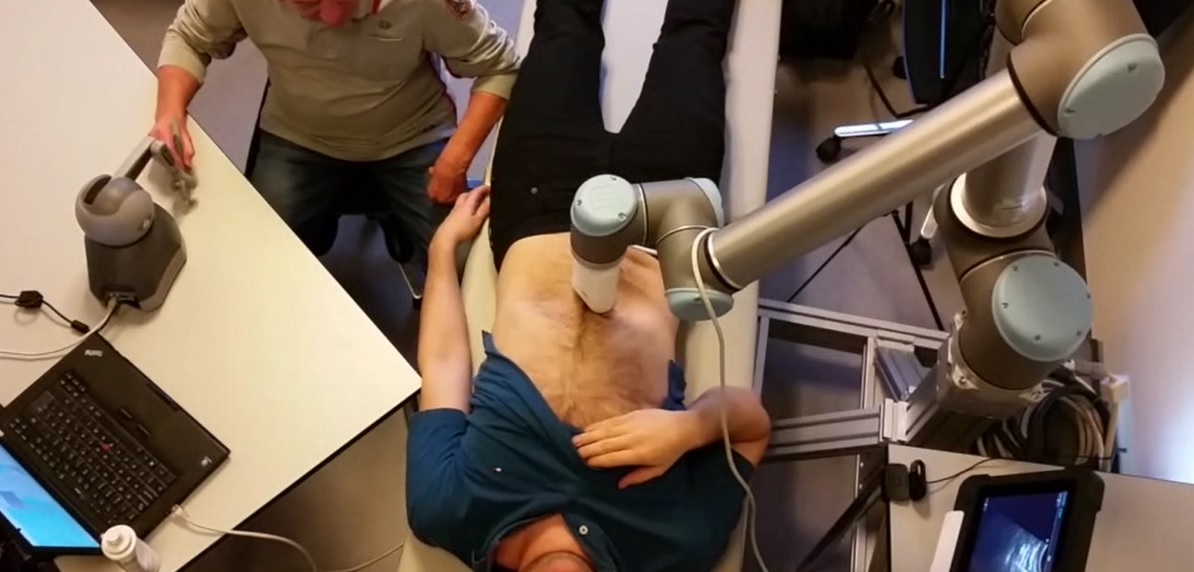
\includegraphics[width = 1.0\textwidth]{Figurer/ergonomiskLosning.jpg}
	\caption{Eksempel på opstilling af Ultralyds Robotarm.}
	\label{ergonomiskLosning}
\end{figure}

\begin{figure}[H]\centering
	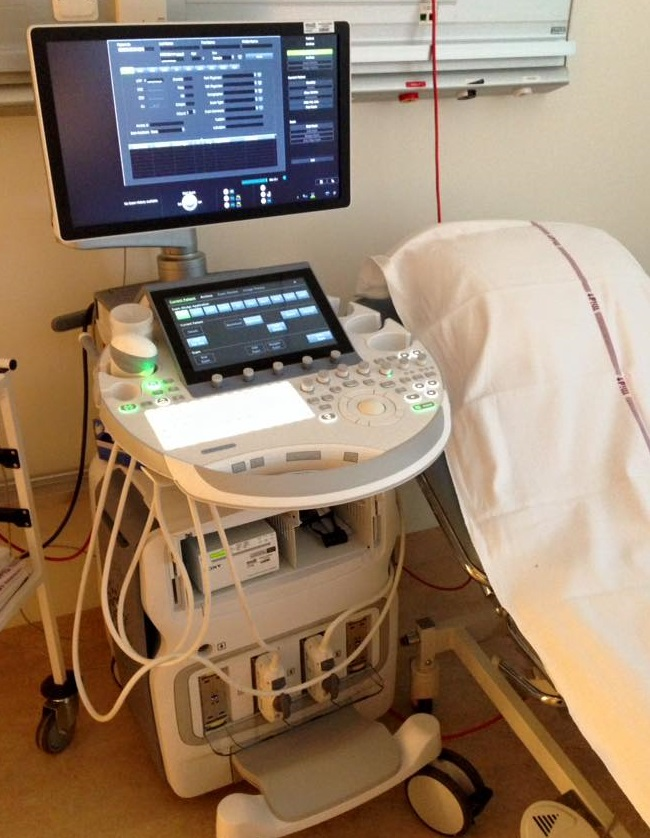
\includegraphics[width = 0.4\textwidth]{Figurer/udstyrHorsens.jpg}
	\caption{Eksempel på ultralydsudstyr fra Horsens.}
	\label{udstyrHorsens}
\end{figure}

\section{Anvendelsesområde}
Produktet skal anvendes til ultralydsscanninger af gravide borgere. Robotarmen sidder på et stativ, som gør at robotarmen kan påvirke med et større tryk, end hvis den blot står ved siden af den gravide. Dette stativ er på hjul, som kan låses, idet systemet skal være mobilt. På robotarmen findes en universalholder til ultralydsproben. Denne holder kan holde alle mærkers ultralydsprobe. \\
Stativet med robotarmen skal være på den modsatte side af sengen, end hvor sonografen er placeret, for at sikre sonografens udsyn og nærkontakt til den gravide.
Robotarmen skal holde ultralydsproben i holderen over den gravide, mens robotarmen styres af sonografen via et joystick. Derved behøver sonografen ikke selv at styre proben og akavede arbejdsstillinger undgås. 
Systemet skal kunne overføre det tryk som sonografen påtrykket joysticket med til robotarmen.
Hvis det tryk, som sonografen påvirker joysticket med, overskrider 15 N (skal lige tjekkes med Søren) slår robotarmen automatisk fra, af sikkerhedsmæssige grunde. 
\begin{figure}[H]\centering
	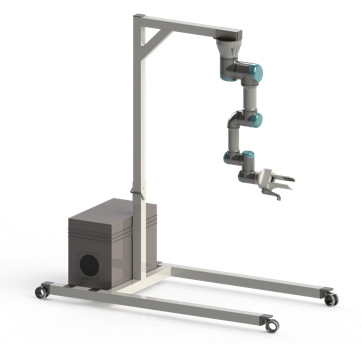
\includegraphics[width = 0.5\textwidth]{Figurer/StativMedUR3Render.png}
	\caption{Skitse af robotarmen på stativet.}
	\label{udstyrHorsens}
\end{figure}
Ultralyds Robotarmen vil kun kunne blive benyttet på 70-80\% af de gravide, da de sidste 20-30\% af scanningerne er for komplicerede til at robotten vil kunne udføre disse. Derfor skal sonografen manuelt foretage de de 20-30\% af scanningerne. De komplicerede ultralydsscanninger er blandt andet på kvinder med høj BMI eller kvinder med bagoverbøjet livmoder. 
\section{Effektivitet}
BMI-problem
Ændrer ikke på produktet - altså samme scanning (der bruges de samme prober)
Tryk - hvordan registreres dette.
\section{Risikovurdering}
pålidelighed
før vs. nu
forbedring af arbejdsstillinger
\section{Delkonklusion}
Ultralyds robotarmen kommer kun til at udføre 70-80\% af scanningerne, hvilket gør at sonograferne stadig skal udføre nogle af scanningerne manuelt. Men at robotarmen kan udføre størstedelen af scanningerne gør, at en stor del af belastningen på sonograferne fjernes. Derfor kan de mest komplicerede scanninger udføres manuelt, da sonograferne vil have mere styrke til disse.

% Kommer sonograferne ud af "træning" - mister styrke??